\documentclass{beamer}
 
\usepackage[utf8]{inputenc}
\usepackage{braket}
\usepackage{mathtools} % Needed for \prescript
\usetheme{boxes}
\setbeamertemplate{navigation symbols}{}
\usepackage{subfig}
\usepackage{hyperref}
\usepackage{xcolor}

\captionsetup[subfigure]{labelformat=empty}
\captionsetup[figure]{labelformat=empty}

\newcommand{\tot}{\mathrm{tot}}
\DeclareMathOperator{\Tr}{Tr}

%Information to be included in the title page:
\title{STIR and Tensorflow}
\author{Philipp Windischhofer}
%\institute{ETH Zürich}
\date{July 27, 2017}
  
\begin{document}
 
\frame{\titlepage}

\begin{frame}
\frametitle{Table of Contents}
\tableofcontents
\end{frame}

\section{Where to start}
\begin{frame}
  \frametitle{The big picture}
  \begin{itemize}
    \item STIR
    \item iterative reconstruction algorithms
      \begin{itemize}
        \item OSMAPOSL
      \end{itemize}
  \end{itemize}
\end{frame}

\section{How to do ray tracing on a CPU?}
\begin{frame}
  \frametitle{How to do ray tracing on a CPU?}
  \framesubtitle{Siddon's algorithm}
\end{frame}

\section{How to do ray tracing on a GPU?}
\begin{frame}
  \frametitle{How to do ray tracing on a GPU?}
  
\end{frame}

\section{Results}
\begin{frame}
  \frametitle{Ray marching: an iterative algorithm}
  \framesubtitle{Accuracy}
  \begin{itemize}
    \item assume: have ``enough'' points along the LOR
  \end{itemize}
  \begin{figure}
    \centering
    \subfloat[][]{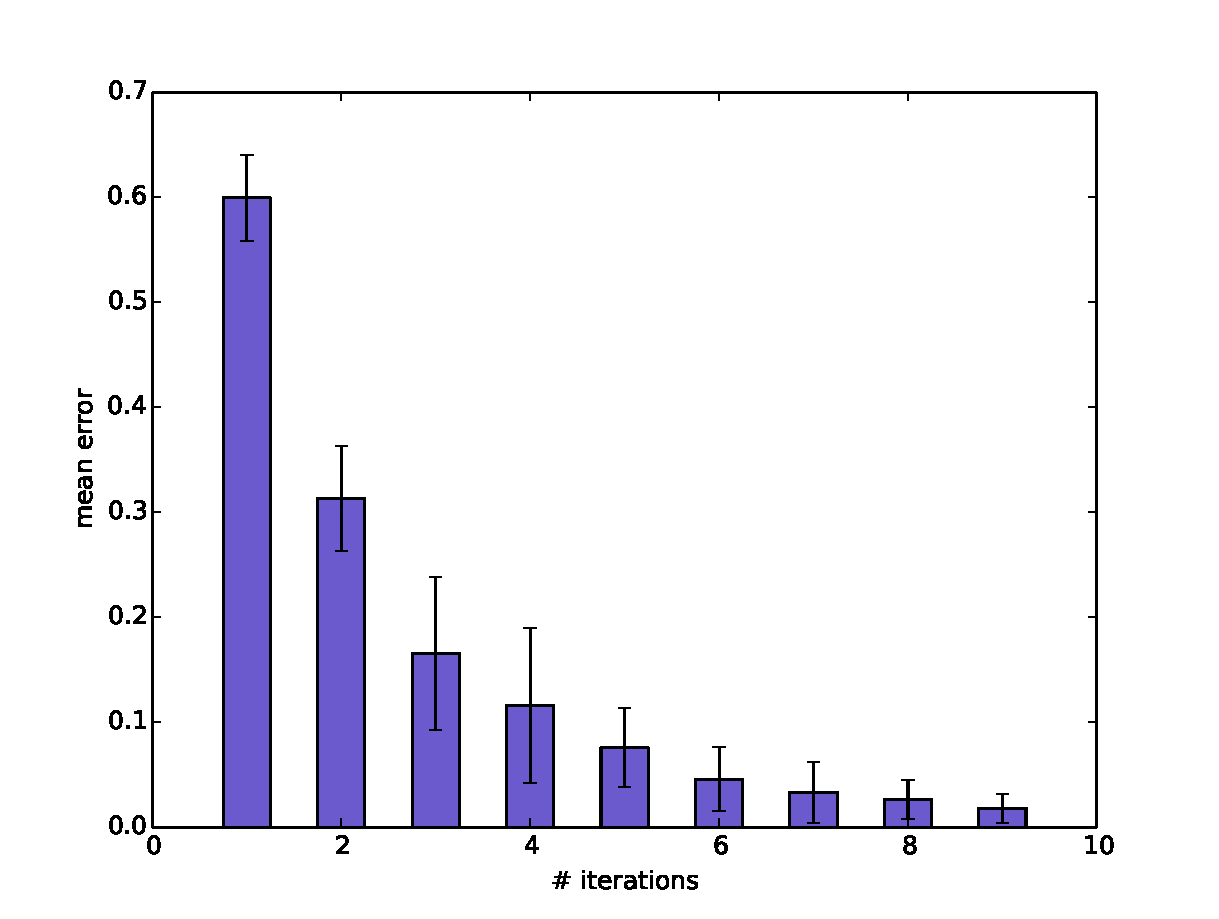
\includegraphics[width = 0.6\textwidth]{../iterations.pdf}\label{6its}}
  \end{figure}
  \begin{itemize}
    \item with 6 iterations, are already at $\sim$ 5\% level!
  \end{itemize}
\end{frame}

\begin{frame}
  \frametitle{Ray marching: an iterative algorithm}
  \framesubtitle{Accuracy}
  \begin{itemize}
    \item are there ever enough points?
  \end{itemize}
  % put 3d histogram here

  \begin{itemize}
    \item does not matter for STIR!
  \end{itemize}
\end{frame}

\begin{frame}
  \frametitle{Bringing together STIR and Tensorflow}
  graph generation in python and graph utilization in c++
\end{frame}

\begin{frame}
  \frametitle{Speedup without caching}
  \begin{figure}
    \centering
      \subfloat[][]{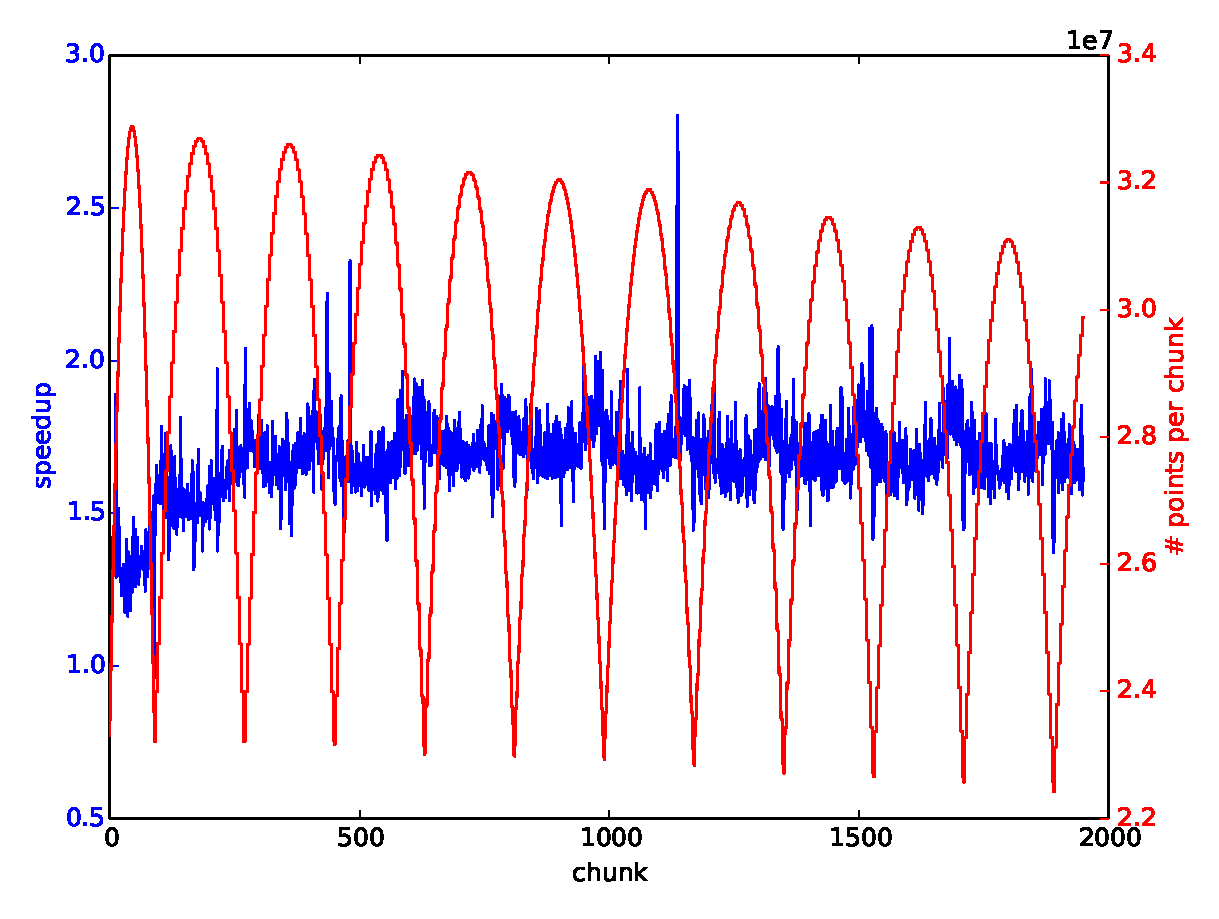
\includegraphics[width = 0.5\textwidth]{../speedup_6_iterations.pdf}\label{6its}}
      \subfloat[][]{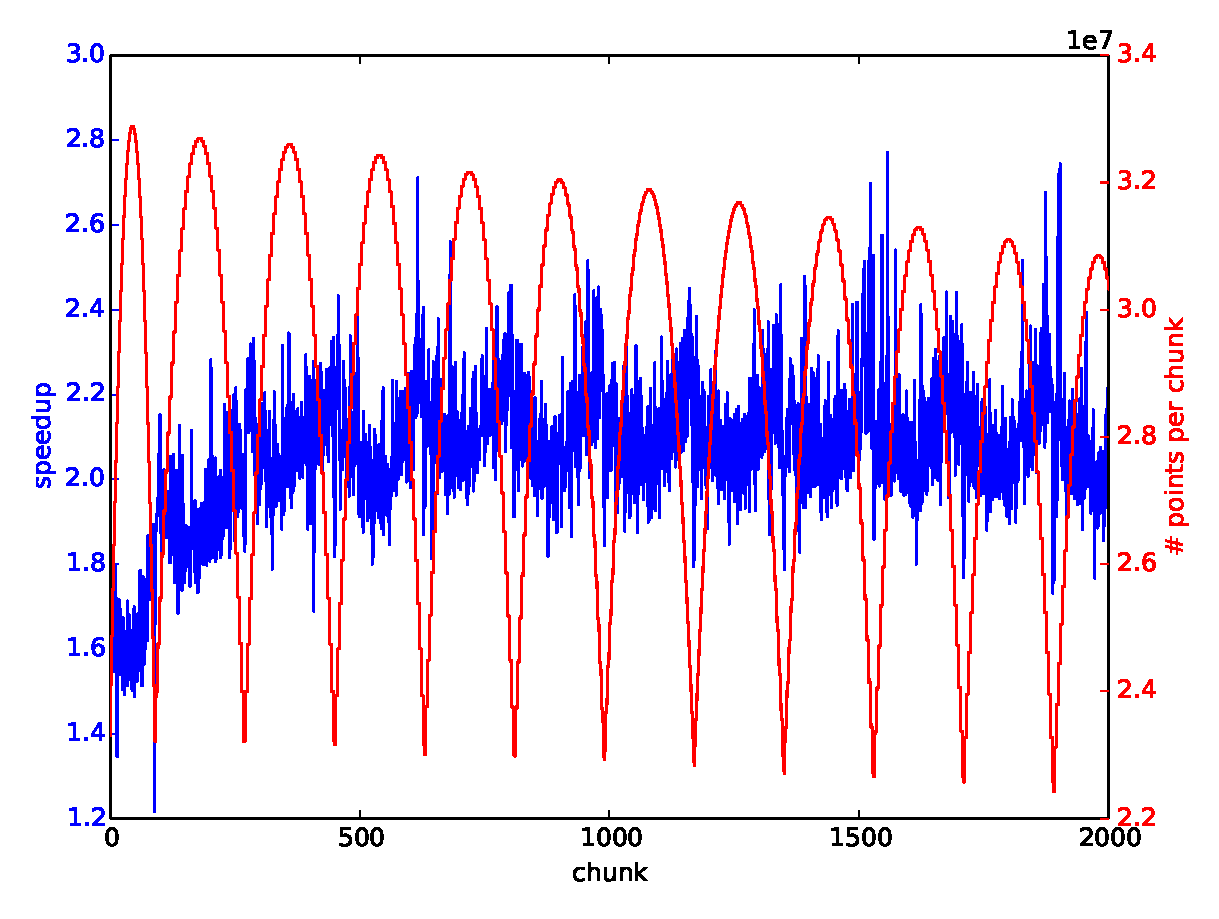
\includegraphics[width = 0.5\textwidth]{../speedup_2_iterations.pdf}\label{2its}}
      \caption{\textbf{left}: 6 iterations, \textbf{right}: 2 iterations}
  \end{figure}
  
  \begin{itemize}
    \item average speedup is similar
  \end{itemize}
\end{frame}

\begin{frame}
  \frametitle{}
  \begin{figure}
    \centering
      \subfloat[][]{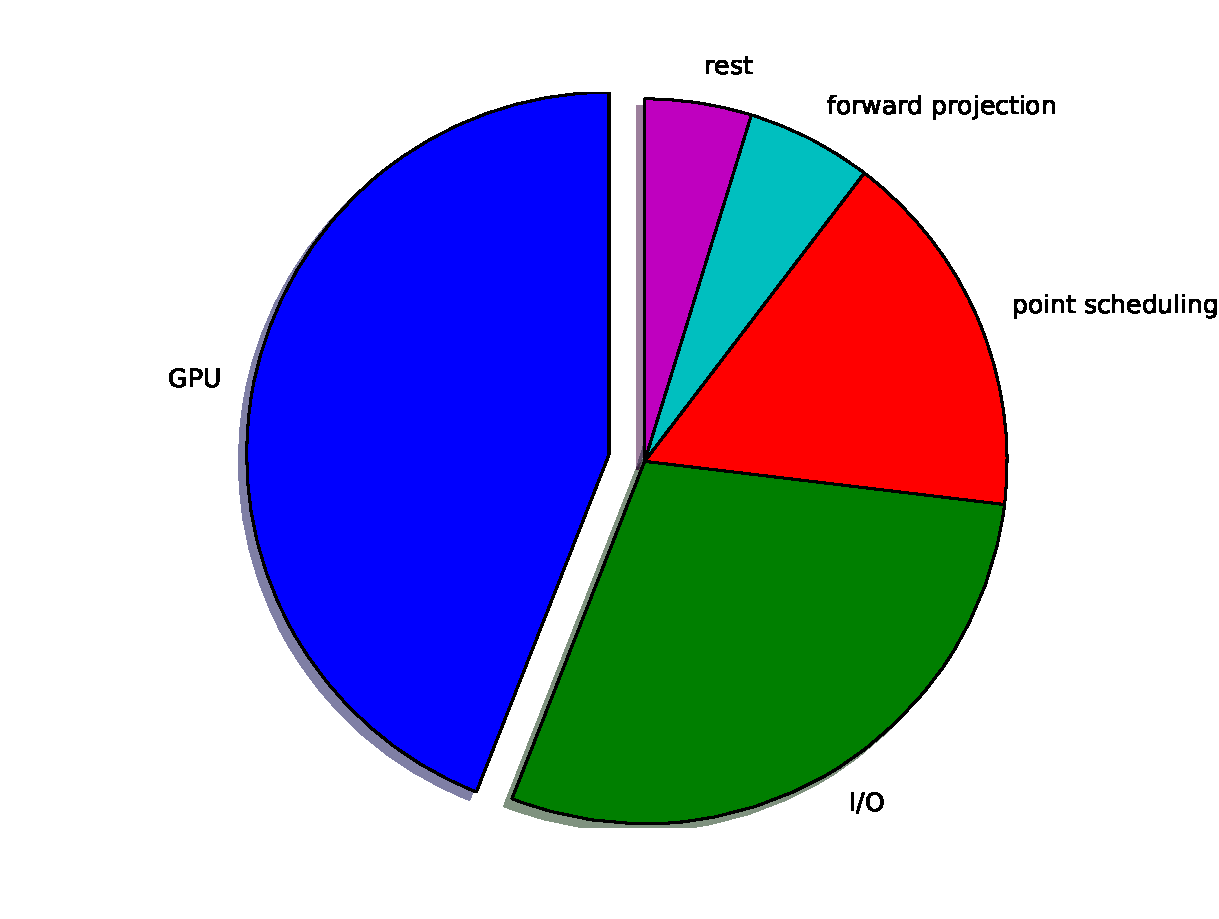
\includegraphics[width = 0.5\textwidth]{../forward_projection_time_distribution_6_iterations.pdf}\label{6its}}
      \subfloat[][]{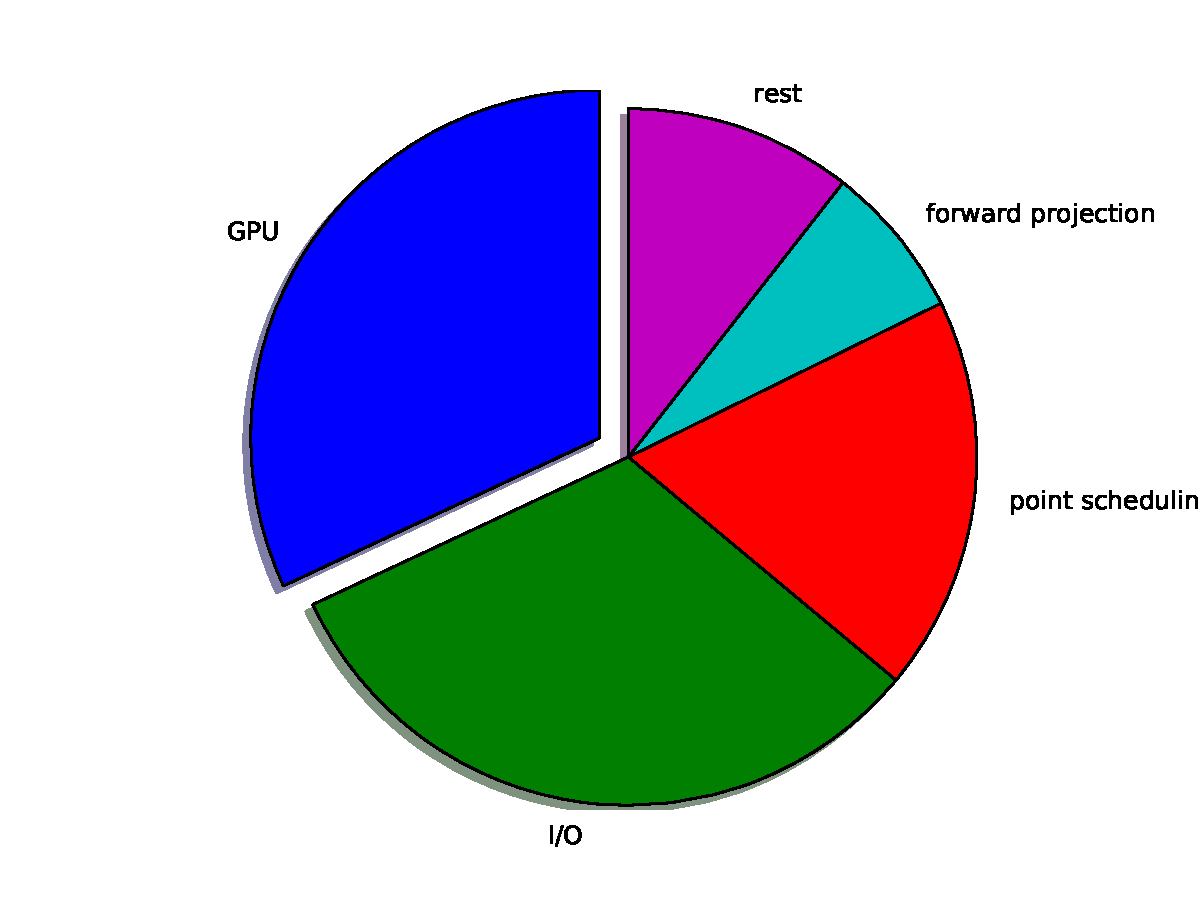
\includegraphics[width = 0.5\textwidth]{../forward_projection_time_distribution_2_iterations.pdf}\label{2its}}
      \caption{\textbf{left}: 6 iterations, \textbf{right}: 2 iterations}
  \end{figure}

  \begin{itemize}
    \item \textsl{I/O}: converting from \texttt{ProjMatrixElemsForOneBin} to \texttt{Tensor} and back
    \item \textsl{point scheduling}: choose points to sample the TOR / LOR
  \end{itemize}
\end{frame}


\begin{frame}
  \frametitle{How to proceed?}
  \begin{itemize}
    \item whole toolchain is in place
  \end{itemize}
\end{frame}

\begin{frame}
  \frametitle{Where to find the code?}
  \begin{itemize}
    \item STIR-TF: \url{https://github.com/philippwindischhofer/STIR/tree/stir-tf}
    \item ray tracing scripts: \url{https://gitlab.phys.ethz.ch/luster/tf-raytracing}
  \end{itemize}

  \begin{center}
    \textcolor{blue}{Any comments and contributions are welcome!}
  \end{center}

\end{frame}

\end{document}
